\clearpage
\part*{Introduction}

L'objectif de ce projet est d'expliquer le fonctionnement des algorithmes de crypto légère (lightweight cryptography).
Il est demandé de choisir deux algorithmes de cryptographie légère, de les expliquer,
de les implémenter et de donner des valeurs de performance aussi bien pour des solutions académiques qu'industrielles.
Il est également demandé de détailler les domaines d'utilisation de ce type d'algorithme.

Une intro

	\clearpage

	% Exemple de code pour ajouter une figure
	% \begin{figure}[h]
	% 	\centering
	% 	\includegraphics[scale=0.8]{imgs/IMAGE.jpg}
	% 	\caption{Définitions géographique de l'espace arctique}
	% 	\label{def_esp_arctic} % le label sert à citer cette figure dans le texte
	%														C'est une genre de référence
	% \end{figure}

	\newpage

\newpage
\part{Introduction à la cryptographie légère}



	\section{Généralités}
	La cryptographie légère est une branche de la cryptographie apparue assez récemment,  et s’étant peu à peu démocratisée au cours de ces vingt dernières années.
	Sa création est née d’un besoin de sécuriser des appareils informatiques de plus en plus petits et de plus en plus nombreux.
	Aujourd’hui, en 2018, on peut dénombrer  plus de  quinze milliards d’objets connectés [5], et ces produits nécessitent d’être sécurisés.
	Si les ordinateurs et mêmes les smartphones de dernière génération offrent une puissance de calcul permettant d’implémenter facilement les algorithmes de cryptographie standard,
	comme par exemple celui du standard AES (algorithme Rinjdael [7]) ou encore RSA,
	ce n’est pas le cas pour les objets les moins puissants et les plus petits comme par exemple les puces RFID,
	certains systèmes embarqués ou les réseaux de capteurs (aussi connus sous leur nom anglais « Sensors Networks ») [6].
	Cette impossibilité d’utiliser des standards de chiffrement « lourds » provient en effet d’un manque de puissance de calcul mais aussi dans la plupart de cas d’un manque d’espace, aussi bien physique que mémoire.  

	On comprend alors l’objet et les enjeux de la cryptographie légère : sécuriser, au moyen d’algorithmes moins coûteux, que ce soit en termes de temps d’exécution ou d’espace mémoire,
	l’ensemble des systèmes informatiques actuels qui ne peuvent être couverts par les standards de la cryptographie « traditionnelle ». 

	\section{Les différences entre cryptographie « traditionnelle » et cryptographie légèrele}
	Avant de commencer la présentation des algorithmes de cryptographie légère que nous avons choisi d’implémenter,
	nous pensons qu’il est de bon ton de décrire les éléments qui permettent de différencier cryptographie légère et « traditionnelle ».

	Commençons par les algorithmes de chiffrement par bloc, dont AES fait partie,
	au même titre que PRESENT qui sera évoqué dans la partie 2 mais qui lui fait partie des algorithmes de cryptographie légère.
	Ces derniers se démarquent des algorithmes de cryptographie standard d’abord par des tailles de bloc plus petites. Là où AES utilise des blocs de 128 bits [7],
	le chiffrement par blocs en cryptographie légère fait le plus souvent appel à des blocs de 64 ou 80 bits [6].
	De même, les clés utilisées sont elles aussi plus courtes : 128, 192 ou 256 bits pour AES [7]  tandis que l’algorithme PRESENT par exemple utilise des clés de 80 bits [2].
	De plus, les rondes de ces algorithmes sont simplifiées, avec notamment des « S-Box » de quatre bits au lieu de huit dans la plupart des algorithmes légers.
	Cela se traduit notamment par un espace physique requis plus faible.	
	En effet, la S-Box de l’AES nécessite 395 GE [8] (« gate equivalents ») alors que la S-Box utilisée par PRESENT n’en nécessite que 28.
	Pour rappel, le « gate equivalent » est une unité de mesure utilisée en électronique qui permet de spécifier la complexité des circuits électroniques en indiquant un nombre de portes logiques nécessaires à la réalisation d’une fonction.
	Le constructeur pourra alors avec ce GE savoir l’espace physique nécessaire pour réaliser ladite fonction [9].
	Pour vous donner une idée plus précise des ordres de grandeur mis en jeu, on peut noter qu’une puce RFID possède une surface généralement comprise entre 1000 et 10000 GE,
	et seulement 200 à 2000 sont dédiées à la sécurité [6]. Enfin, les algorithmes de chiffrement par blocs en cryptographie légère implémentes des opérations sur les clés de chiffrement beaucoup plus simples et beaucoup moins coûteux qu’en cryptographie standard.

	D’autre part, intéressons-nous cette fois aux algorithmes de hachage.
	Tout d’abord, la principale différence réside dans la taille des états internes et des hachés produits par l’algorithme.
	Par exemple, SHA-2 sort des hachés de 256 bits tandis que SPONGENT (algorithme présenté dans la deuxième partie) retourne des hachés qui peuvent descendre jusqu’à 88 bits [1].
	De plus, une autre différence entre ces algorithmes de hachage se situe dans la taille des messages en entrée des algorithmes.
	Là où des algorithmes standards peuvent travailler sur des messages très grands (264 bits), les algorithmes de hachage de cryptographie légère travaillent sur des données d’entrée beaucoup plus faibles, plutôt de l’ordre de $2^8$ bits.

	Enfin, il faut tout de même noter que la cryptographie légère n’a pas que des avantages face à la cryptographie traditionnelle.
	En effet, réduire les tailles des blocs, des clés, a un coût en termes de sécurité.
	Par exemple, l’utilisation de blocs de 64 bits dans certains algorithmes réduit considérablement le nombre de sorties possibles d’un algorithme,
	et dans ces cas-là un chiffré peut-être différencié d’une séquence aléatoire en utilisant seulement 232 blocs.
	Il en résulte alors que certains algorithmes sont vulnérables aux attaques de type « plaintext recovery » ou « key recovery » avec des probabilités non négligeables.


\part{Présentation de deux algorithmes de cryptographie légère}

	\section{SPONGENT}
	Cette partie a pour objectif de présenter l’algorithme de cryptographie légère SPONGENT.
	Il découle directement de l’algorithme PRESENT, développé en 2007 par « Orange Labs », la « Ruhr University Bochum » et la « Technical  University of Denmark ».
	Ce dernier est un algorithme par blocs (de 64 bits) dont la clé fait 80 ou 128 bits [2],
	et il a la particularité d’avoir été inclus au dernier standard international des méthodes de cryptographie légère par l’ « International Electrotechnical Commission » [3].

		\subsection{Fonctionnement général de SPONGENT}

		\begin{figure}[h]
			 	\centering
			 	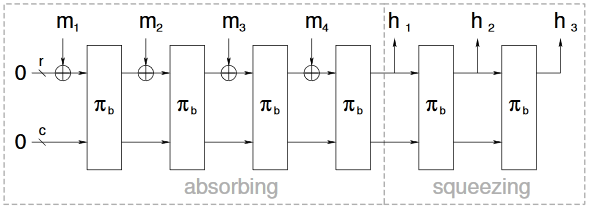
\includegraphics[scale=0.8]{imgs/Spongent/fctGlobalSpongent.png}
			 	\caption{Schéma illustrant le fonctionnement de SPONGENT, tiré de [1]}
			 	\label{fctGlobalSpongent}
		\end{figure}

		Comme énoncé précédemment, SPONGENT s’appuie sur le fonctionnement de l’algorithme PRESENT.
		Pour un nombre fini de bits en entrée, SPONGENT va produire un hach de taille n (fixé).
		La figure \ref{fctGlobalSpongent} schématise le fonctionnement de l’algorithme, qui s’organise en trois phases distinctes, que sont l’initialisation, l’absorption (absorbing) et le relâchement (squeezing).

		L’initialisation consiste à ajouter un 1 binaire suivi de x 0 afin que la taille du message en entrée soit un multiple de la taille des blocs, appelé r (rate en anglais).
		Le message est ensuite découpé en blocs de r bits.
		Ensuite vient la phase d’absorption.
		Durant cette phase, un bloc mi subit un XOR avec les r premiers bits de l’état courant et passe ensuite dans la fonction de permutation.
		Cette permutation génère un état de b bits, où $b = r + c$, et où c est appelé la capacité de l’état et b est appelé la largeur de l’état.
		Enfin, la phase de relâchement consiste à retourner les r premiers bits de l’état, puis de passer l’état dans la fonction de permutation,
		et de répéter ces deux opérations jusqu’à ce que le hach retourné ait une longueur de n bits.

		Les valeurs de n, b, c et r ne sont pas prises au hasard. En effet, il existe treize versions différentes de SPONGENT et elles sont définies grâce au tableau représenté à la figure \ref{variantesSpongent}.
		Ces treize versions s’appuient sur des hachés de tailles différentes, mais les valeurs des trois autres constantes citées ci-avant diffèrent elles-aussi selon la version utilisée.
		Dans le cas de notre projet, nous avons décidé d’implémenter SPONGENT 160/160/80.
		
		\begin{figure}[h]
			\centering
			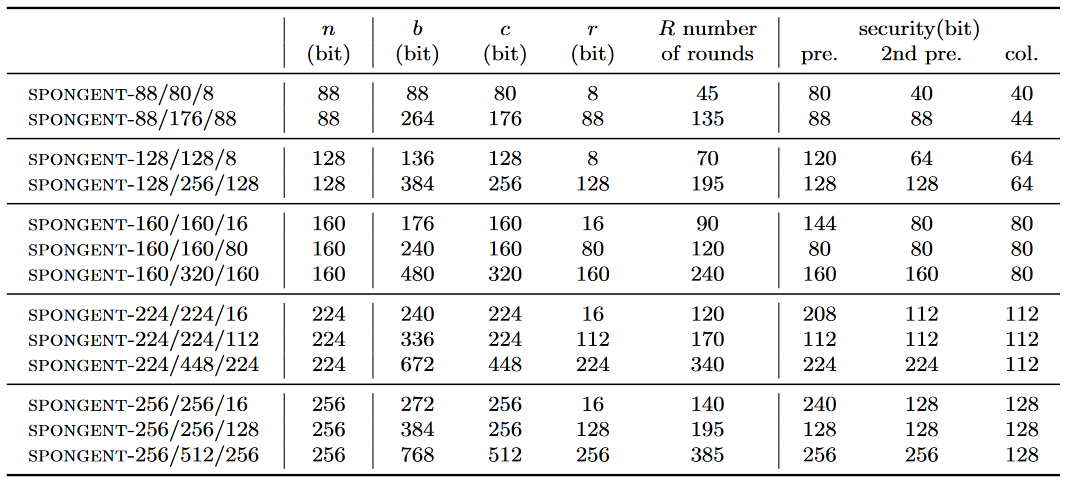
\includegraphics[width=\textwidth]{imgs/Spongent/varianteSpongent.png}
			\caption{Tableau définissant  les 13 variantes de SPONGENT, tiré de [1]}
			\label{variantesSpongent}
   		\end{figure}

		\subsection{Fonctionnement détaillé de SPONGENT 160 / 160 / 80}
		Cette sous-partie va permettre d’expliquer le fonctionnement détaillé de la permutation notée $\pi_{b}$.
		Cette permutation est définie par l’algorithme \ref{algoSpongent}:
		\begin{algorithm}
			\caption{Algorithme de permutation de SPONGENT}
			\label{algoSpongent}
			\begin{algorithmic}
				\FOR{i = 1 to R}
					\STATE $ STATE \leftarrow lCounter_{b}(i) \xor STATE \xor lCounter_{b}(i)$
					\STATE $ STATE \leftarrow sBoxLayer_{b}(STATE)$
					\STATE $ STATE \leftarrow pLayer_{b}(STATE)$
				\ENDFOR
			\end{algorithmic}
		\end{algorithm}

		Tout d’abord, intéressons-nous aux variables de cet algorithme.
		La variable R est le nombre de rondes de l’algorithme. Il varie en fonction de la variante de SPONGENT utilisée, et dans notre cas R vaut 80.
		Ensuite, la variable STATE représente l’état courant.
		
		La première opération appliquée à STATE est un XOR avec d’une part lCounterb(i) et d’autre part la valeur « retournée » de lCounterb(i),
		c’est-à-dire que si lCounterb(i) = 1000 sa valeur « retournée » est 0001. lCounterb(i) est en réalité un LFSR, ou Registre à décalage à rétroaction linéaire,
		soit un générateur pseudo-aléatoire qui dépend lui aussi de la variante de l’algorithme utilisée.
		La figure \ref{polyPrimitifsLFSR} illustre les polynômes générateurs du LFSR, et la figure \ref{valInitLFSR} indique les valeurs initiales que prend le LFSR.

		\begin{figure}[!htb]
			\begin{minipage}{0.48\textwidth}
			  \centering
			  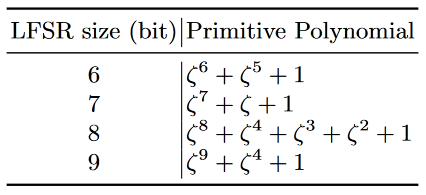
\includegraphics[width=\textwidth]{imgs/Spongent/PrimiPolySpongent.png}
			  \caption{Polynômes primitifs du LFSR}
			  \label{polyPrimitifsLFSR}
			\end{minipage}
			\hfill
			\begin {minipage}{0.48\textwidth}
			  \centering
			  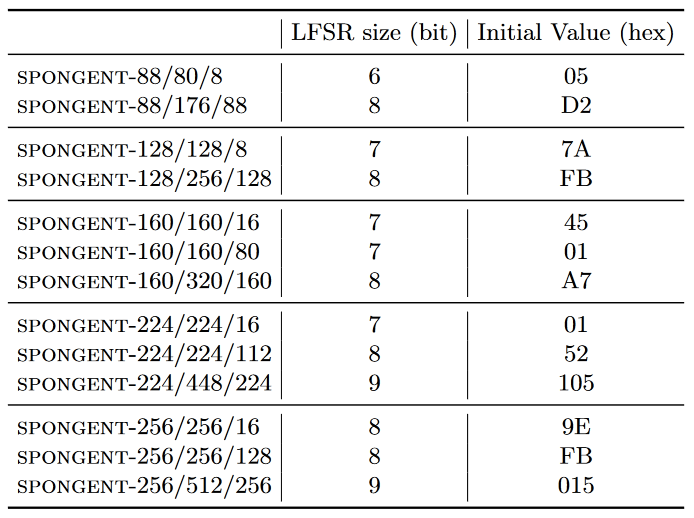
\includegraphics[width=\textwidth]{imgs/Spongent/valInitLFSR.png}
			  \caption{Valeurs initiales du LFSR}
			  \label{valInitLFSR}
			\end{minipage}
		 \end{figure}
		La deuxième opération de la ronde est de passer STATE dans une S-Box.
		La S-Box est la même pour toutes les variantes de l’algorithme SPONGENT et elle est définie par la figure \ref{sBoxSpongent.png} :
		
		\begin{figure}[h]
			\centering
			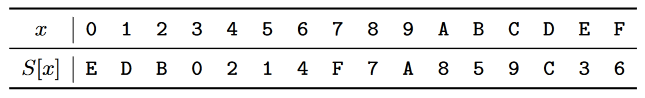
\includegraphics[width=\textwidth]{imgs/Spongent/sBoxSpongent.png}
			\caption{S-Box de l'algorithme SPONGENT}
			\label{sBoxSpongent.png}
		\end{figure}
		   
		Enfin, la troisième et dernière opération est de passer STATE dans $pLayer_{b}$.
		$pLayer_{b}$ est une fonction de permutation définie comme l’inverse de la permutation de bits de l’algorithme PRESENT.
		Ainsi, chaque bit j est permuté avec le bit de position $P_{b}(j)$ où :

		\begin{figure}[htbp]
			\centering
		\begin{equation}
			P_{b}(j) = \begin{cases}
			  j \cdot \frac{b}{4} \bmod b - 1, if j \in {0, \dots, b - 2}\\
			  b - 1, \text{if j = b - 1}.
			\end{cases}
		  \end{equation}
		  \caption{Formule de permutation de pLayer}
			\label{pLayer}
		\end{figure}

		\subparagraph{Performances et sécurité}

		Les variantes de SPONGENT peuvent être implémentées en utilisant entre 738 GE (pour SPONGENT 80/80/8) et 5100 GE (pour SPONGENT 256/512/256).
		Ces nombres ne semblent peut-être pas très explicites, mais ils dénotent une très grande compacité de l’implémentation physique de l’algorithme.
		Pour plus de détails, la figure \ref{espacePhysique} présente pour différentes variantes de l’algorithme l’espace physique nécessaire en fonction de la technologie (NXP, UMC et NANGATE)[11] :

		\begin{figure}[h]
			\centering
			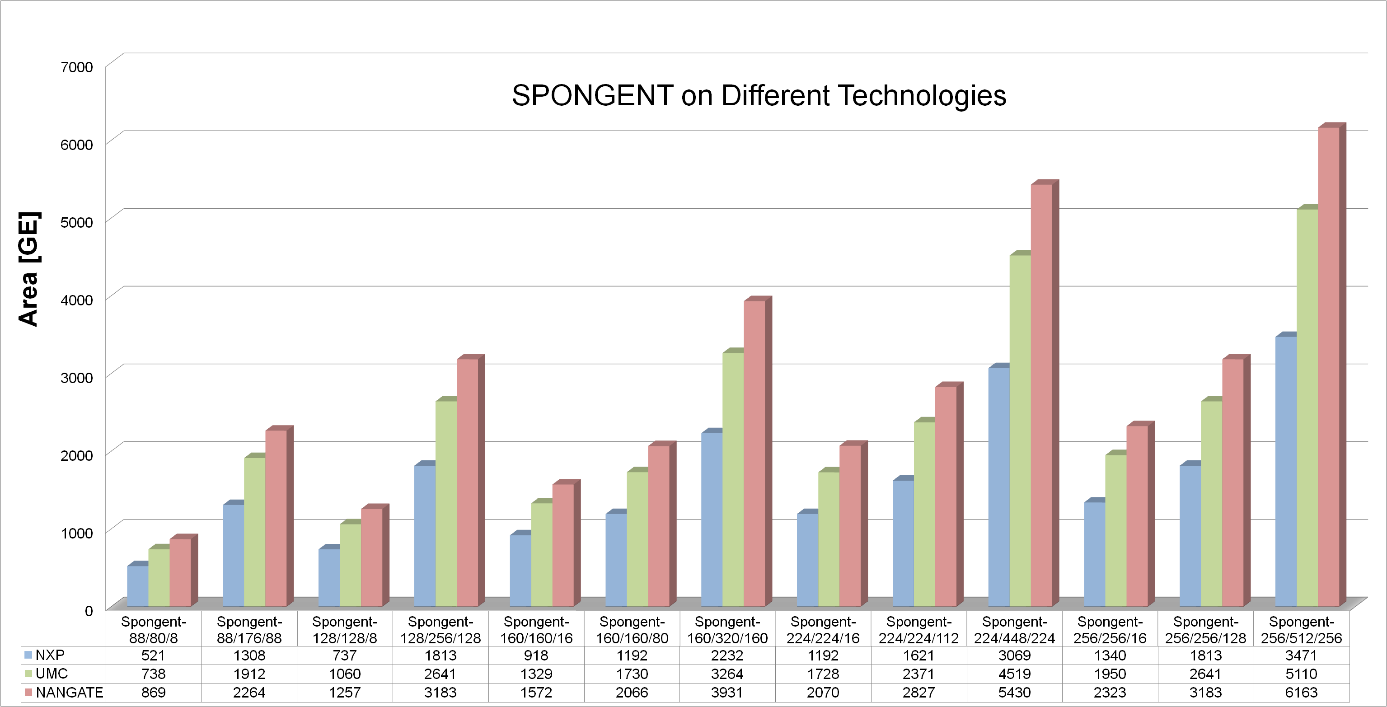
\includegraphics[width=\textwidth]{imgs/Spongent/espacePhysiqueVariante.png}
			\caption{Espace physique nécessaire pour différentes variantes de SPONGENT}
			\label{espacePhysique}
		\end{figure}

		Pour ce qui est du débit de traitement, il est donné comme variant entre 360 Mbps et 2 Gbps (en fonction de la variante de SPONGENT utilisée).
		En comparaison, l’algorithme de hachage SHA-1 possède un débit de l’ordre d’ 1 Gbps [10].

		\begin{figure}[h]
			\centering
			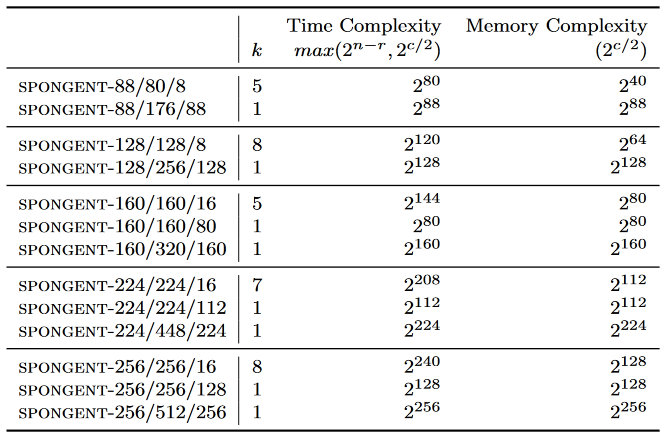
\includegraphics[width=\textwidth]{imgs/Spongent/timeComplexity.png}
			\caption{Complexités en temps et en mémoire de SPONGENT}
			\label{timeComplexity}
		\end{figure}

		En termes de sécurité, nous pouvons voir sur la figure \ref{timeComplexity} les différentes valeurs de complexité pour l’ensemble des variantes de SPONGENT.
		Pour les variantes 88/80/8 et 128/128/8, il est intéressant de noter que nous sommes dans des capacités de calcul atteignables, et que de ce fait ces algorithmes ne sont pas « sûrs ».
		Pour le reste, nous pouvons observer des complexités relatives au minimum inatteignable ($2^{80}$) voire raisonnablement inatteignable ($2^{128}$).
		
		Enfin, la figure \ref{attaquePreImage} présente les résultats de sécurité face aux attaques par pré-image, par 2\up{ème} pré-image et par collision [11].
		L’attaque par pré-image consiste, à partir d’un haché $y$, à retrouver un $x$ tel que $h(x) = y$.
		L’attaque par 2\up{ème} pré-image consiste quant à elle, à partir d’un clair $x$, à trouver $x’$ tel que $h(x) = h(x’)$.
		Enfin, l’attaque par collision consiste à essayer de trouver deux clairs différents produisant le même chiffré.
		Elle ressemble à l’attaque par 2\up{ème} pré-image à ceci près que le clair n’est pas spécifié.
		
		\begin{figure}[h]
			\centering
			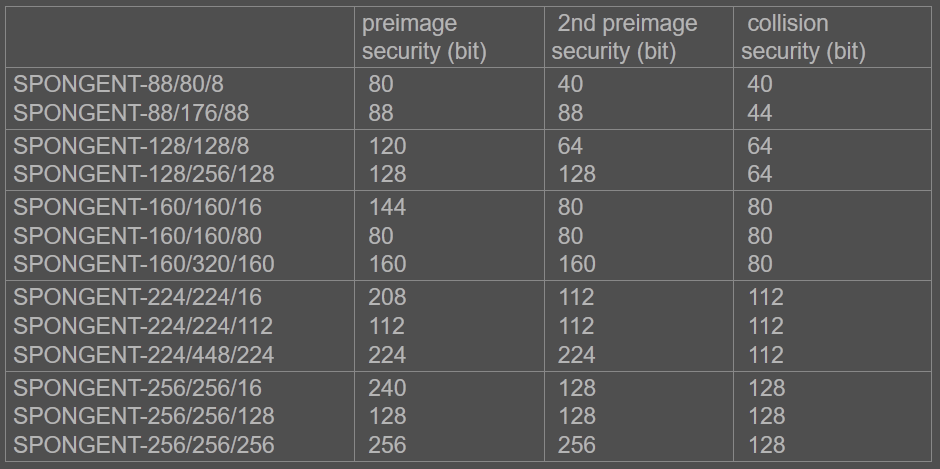
\includegraphics[width=\textwidth]{imgs/Spongent/attaquePreImage.png}
			\caption{Attaque par pré-image et collision}
			\label{attaquePreImage}
		\end{figure}

		%% TODO : integrer la biblio dans biber

		\section{Speck}

			Speck est un algorithme de chiffrement par bloc léger crée par la NSA et rendu
		publique en 2013. C'est un algorithme spécialement conçu pour avoir des performances
		élevées afin d'offrir un algorithme de chiffrement utilisable dans le cadre de
		"l'Internet of Things".

		\subsection{Algorithmes ARX}

				Cet algorithme fait parti des algorithmes dits ARX, Add-Rotate-Xor. C'est une famille
			d'algorithmes qui n'utilisent que les opérations d'additions, rotations et ou exclusif
			dans l'espace $GF_{2^n}$. Il y a plusieurs avantages à se limiter à ces opérations:

			\begin{enumerate}
			\item[•] Rapidité: ces opérations sont des opérations logiques. Ainsi, elles sont
				des primitives de tout micro-controlleur et donc sont effectué en un seul
				cycle d'horloge.
			\item[•] Sécurité matérielle: le fait que toutes les opérations soient des opérations
				logiques atomiques permet à ces algorithmes de fonctionner en temps constant.
				Prévenant les attaques par canaux cachés basés sur les mesures de temps.
			\item[•] Implémentation: ces algorithmes sont souvent très simples. Leur implémentation
				qu'elle soit logicielle ou matérielle est très simple. Par conséquent, le
				temps de développement et le coût de leur implémentation est très faible.
			\end{enumerate}

		\subsection{Fonctionnement de Speck}

			Avant de détailler comment fonctionne Speck, considérons les notations suivantes:

			\begin{enumerate}
			  \item[•] Le ou-exclusif bit à bit, noté xor
			  \item[•] L'addiction modulo $2^n$, noté $\xor$
			  \item[•] Les rotations circulaires à gauche et à droite respectivement notées,
			    $S^i$ et $S^{-i}$ pour des rotations de i-bits.
			\end{enumerate}

			Un tour de chiffrement de l'algorithme Speck est définit de la façon suivante. \\
			Pour $k \in GF(2^n)$ une clée, le tour de chiffrement est définit par la fonction suivante:
			\[
			\begin{array}{ccccc}
			R_k & : & GF(2^n) x GF(2^n) & \to & GF(2^n) x GF(2^n) \\
			 & & (x,y) & \mapsto & ((S^{-\alpha}(x) + y) \xor k, S^\beta (y) \xor (S^{-\alpha} + y) \xor k) \\
			\end{array}
			\]

			avec $\alpha$ = 7 et $\beta$ = 2 si n = 16, $\alpha $= 8 et $\beta$ = 3 sinon. \\

			La fonction de déchiffrement est définie par:
			\[
			\begin{array}{ccccc}
			R_k^{-1} & : & GF(2^n) x GF(2^n) & \to & GF(2^n) x GF(2^n) \\
			 & & (x,y) & \mapsto & (S^\alpha ((x \xor k) - S^{-\beta}(x \xor y)), S^{-\beta}(x \xor y)) \\
			\end{array}
			\]


\newpage
\part*{Conclusion}

		La conlusion
